\documentclass[tikz,border=8pt]{standalone}
\usepackage{fontspec}
\usepackage{xeCJK}
\usetikzlibrary{calc}

\setmainfont{Times New Roman}
\setsansfont{Arial}
\setCJKmainfont{DFKai-SB.ttf}

\definecolor{ink}{HTML}{243044}
\definecolor{muted}{HTML}{637083}
\definecolor{line}{HTML}{7B8798}
\definecolor{inputColor}{HTML}{6E7787}
\definecolor{blue}{HTML}{2563A9}
\definecolor{blueFill}{HTML}{D8EEF9}
\definecolor{labelBlue}{HTML}{1E5B93}
\definecolor{labelGreen}{HTML}{188451}
\definecolor{teal}{HTML}{18A7A7}
\definecolor{tealFill}{HTML}{D8F3F0}
\definecolor{green}{HTML}{21A85A}
\definecolor{greenFill}{HTML}{DDF6E5}
\definecolor{softmaxFill}{HTML}{CFF7D6}
\definecolor{bnColor}{HTML}{F6C85F}
\definecolor{reluColor}{HTML}{76B7B2}
\definecolor{dropColor}{HTML}{E15759}
\definecolor{opFill}{HTML}{D8EEF9}
\definecolor{opLine}{HTML}{2563A9}

\tikzset{
    inputnode/.style={
        circle,
        draw=inputColor,
        fill=white,
        line width=0.8pt,
        minimum size=5.6pt,
        inner sep=0pt
    },
    hiddennode/.style={
        circle,
        draw=blue,
        fill=blueFill,
        line width=0.9pt,
        minimum size=8.5pt,
        inner sep=0pt
    },
    outputnode/.style={
        circle,
        draw=green,
        fill=greenFill,
        line width=1.0pt,
        minimum size=9pt,
        inner sep=0pt
    },
    probnode/.style={
        circle,
        draw=green,
        fill=softmaxFill,
        line width=1.0pt,
        minimum size=8.5pt,
        inner sep=0pt
    },
    connect/.style={
        draw=line,
        line width=0.24pt,
        opacity=0.20
    },
    mainarrow/.style={
        ->,
        draw=ink!72,
        line width=0.9pt
    },
    softmaxarrow/.style={
        ->,
        draw=green!70!black,
        line width=0.95pt,
        opacity=0.90
    },
    layerlabel/.style={
        font=\sffamily\fontsize{12.4}{14.4}\selectfont\bfseries,
        text=labelBlue,
        align=center
    },
    softmaxlabel/.style={
        font=\sffamily\fontsize{12.2}{14.2}\selectfont\bfseries,
        text=labelGreen,
        align=center
    },
    layernote/.style={
        font=\sffamily\fontsize{9.4}{11}\selectfont,
        text=muted,
        align=center
    },
    classlabel/.style={
        font=\sffamily\fontsize{10.8}{12.8}\selectfont,
        text=ink,
        anchor=west
    }
}

\begin{document}
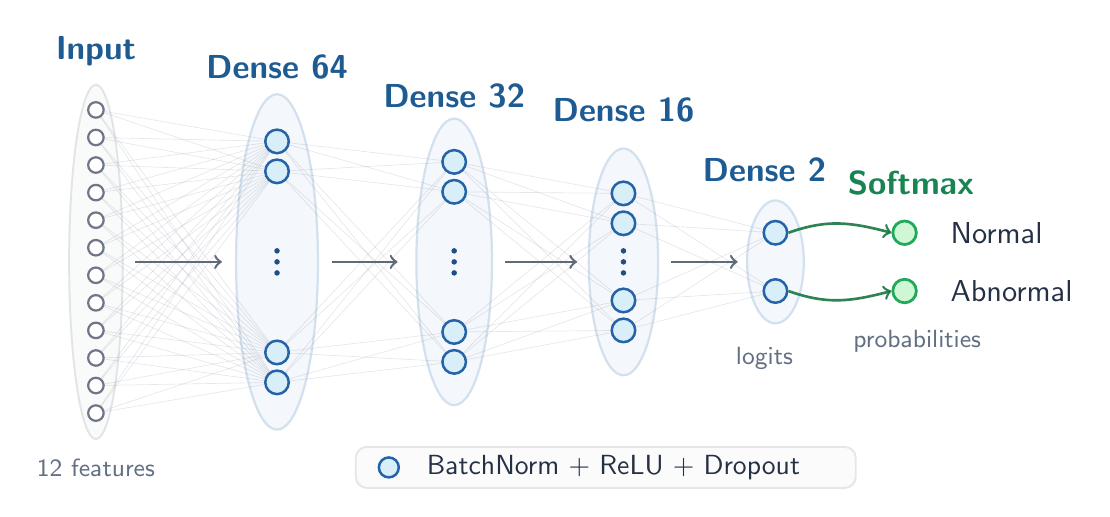
\begin{tikzpicture}[x=1cm,y=1cm]
    % Layer backgrounds
    \filldraw[fill=inputColor!4, draw=inputColor!20, line width=0.7pt]
        (0.75,2.55) ellipse [x radius=0.34, y radius=2.25];
    \filldraw[fill=blue!5, draw=blue!20, line width=0.8pt]
        (3.05,2.55) ellipse [x radius=0.52, y radius=2.13];
    \filldraw[fill=blue!5, draw=blue!20, line width=0.8pt]
        (5.30,2.55) ellipse [x radius=0.48, y radius=1.82];
    \filldraw[fill=blue!5, draw=blue!20, line width=0.8pt]
        (7.45,2.55) ellipse [x radius=0.44, y radius=1.44];
    \filldraw[fill=blue!5, draw=blue!20, line width=0.8pt]
        (9.38,2.55) ellipse [x radius=0.36, y radius=0.78];

    % Input: exactly 12 features
    \foreach \i in {1,...,12} {
        \pgfmathsetmacro{\y}{4.48-(\i-1)*0.35}
        \node[inputnode] (input-\i) at (0.75,\y) {};
    }

    % Dense 64 representation: visible units with ellipsis for omitted units
    \node[hiddennode] (h1-1) at (3.05,4.08) {};
    \node[hiddennode] (h1-2) at (3.05,3.70) {};
    \foreach \dy in {-0.14,0,0.14} {
        \fill[blue!80!black] (3.05,{2.55+\dy}) circle[radius=0.035];
    }
    \node[hiddennode] (h1-3) at (3.05,1.40) {};
    \node[hiddennode] (h1-4) at (3.05,1.02) {};

    % Dense 32 representation: visible units with ellipsis for omitted units
    \node[hiddennode] (h2-1) at (5.30,3.82) {};
    \node[hiddennode] (h2-2) at (5.30,3.44) {};
    \foreach \dy in {-0.14,0,0.14} {
        \fill[blue!80!black] (5.30,{2.55+\dy}) circle[radius=0.035];
    }
    \node[hiddennode] (h2-3) at (5.30,1.66) {};
    \node[hiddennode] (h2-4) at (5.30,1.28) {};

    % Dense 16 representation: visible units with ellipsis for omitted units
    \node[hiddennode] (h3-1) at (7.45,3.42) {};
    \node[hiddennode] (h3-2) at (7.45,3.04) {};
    \foreach \dy in {-0.14,0,0.14} {
        \fill[blue!80!black] (7.45,{2.55+\dy}) circle[radius=0.035];
    }
    \node[hiddennode] (h3-3) at (7.45,2.06) {};
    \node[hiddennode] (h3-4) at (7.45,1.68) {};

    % Dense 2 logits
    \node[hiddennode] (out-1) at (9.38,2.92) {};
    \node[hiddennode] (out-2) at (9.38,2.18) {};

    % Fully connected relationships, drawn lightly to avoid clutter
    \foreach \i in {1,...,12} {
        \foreach \j in {1,...,4} {
            \draw[connect] (input-\i) -- (h1-\j);
        }
    }
    \foreach \i in {1,...,4} {
        \foreach \j in {1,...,4} {
            \draw[connect] (h1-\i) -- (h2-\j);
        }
    }
    \foreach \i in {1,...,4} {
        \foreach \j in {1,...,4} {
            \draw[connect] (h2-\i) -- (h3-\j);
        }
    }
    \foreach \i in {1,...,4} {
        \foreach \j in {1,...,2} {
            \draw[connect] (h3-\i) -- (out-\j);
        }
    }

    % Main flow arrows
    \draw[mainarrow] (1.25,2.55) -- (2.35,2.55);
    \draw[mainarrow] (3.75,2.55) -- (4.58,2.55);
    \draw[mainarrow] (5.95,2.55) -- (6.86,2.55);
    \draw[mainarrow] (8.05,2.55) -- (8.90,2.55);

    % Softmax probability nodes
    \node[softmaxlabel] at (11.10,3.55) {Softmax};
    \node[probnode] (prob-1) at (11.02,2.92) {};
    \node[probnode] (prob-2) at (11.02,2.18) {};
    \draw[softmaxarrow] (out-1.east) .. controls (10.05,3.10) and (10.35,3.05) .. (prob-1.west);
    \draw[softmaxarrow] (out-2.east) .. controls (10.05,2.00) and (10.35,2.05) .. (prob-2.west);
    \node[classlabel] at (11.48,2.92) {Normal};
    \node[classlabel] at (11.48,2.18) {Abnormal};

    % Labels
    \node[layerlabel] at (0.75,5.22) {Input};
    \node[layernote] at (0.75,-0.06) {12 features};

    \node[layerlabel] at (3.05,5.02) {Dense 64};

    \node[layerlabel] at (5.30,4.66) {Dense 32};

    \node[layerlabel] at (7.45,4.48) {Dense 16};

    \node[layerlabel] at (9.24,3.72) {Dense 2};
    \node[layernote] at (9.24,1.32) {logits};
    \node[layernote] at (11.18,1.54) {probabilities};

    % Legend for repeated hidden-layer operations
    \begin{scope}[shift={(4.05,-0.32)}]
        \filldraw[rounded corners=4pt, fill=ink!2, draw=ink!12, line width=0.7pt]
            (0,0) rectangle (6.35,0.52);
        \node[hiddennode, minimum size=7.2pt] at (0.42,0.26) {};
        \node[font=\sffamily\fontsize{10.2}{12}\selectfont, text=ink, anchor=west]
            at (0.78,0.26) {BatchNorm + ReLU + Dropout};
    \end{scope}

\end{tikzpicture}
\end{document}
